\subsection{Funcionamiento del LM35}
El LM35 es sensor de temperatura que viene en forma de un integrado con 3 terminales. El funcionamiento es simple, se alimenta al integrado por su terminal de entrada $V_s$ con una fuente de tensión continua de $4V$ a $20V$, luego en su terminal de salida $V_o$ devolverá $10mV$ por cada $°C$ que el sensor detecte en el ambiente.

\begin{equation}
    V_T(T) = 0mV + \frac{10 mV}{°C} T
\end{equation}


Si el sensor está en un ambiente (o se lleva al integrado a tal temperatura) a $0°C$ devolverá $0V$, mientras que a $35°C$ devolverá $350mV$ y a $45°C$ devolverá $450mV$.



\subsection{Implementación en rango de 35°C y 45°C}

El objetivo es poder adaptar una señal para que pueda ser adquirida con máxima excursión para temperaturas que varíen entre 35°C y 45°C (siendo 35°C correspondiente con 0V y 45°C correspondiente con 5V).

Para esto utilizamos un amplificador operacional LM833 y usamos un circuito sumador de dos señales, donde la primer señal $V_i$ será la emitida por el LM35 y la segunda señal será una fuente de tensión continua que servirá para imponer un offset ($V_f$) ya que buscamos que la salida de $0V$ corresponda a los $35°C$ y no a los $0°C$. Utilizando el siguiente esquema podemos analizarlo y estudiar como serán las relaciones de las resistencias que necesitamos:

\begin{figure}[H]
    \centering
    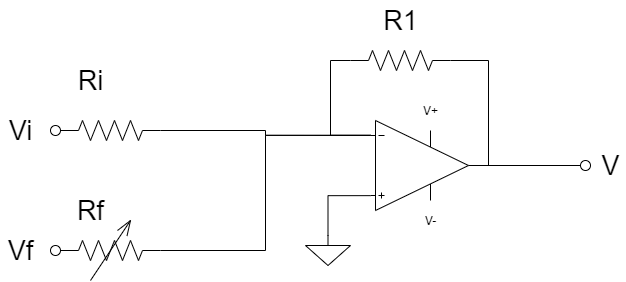
\includegraphics[scale=0.5]{../Ejercicio4-CircuitodeAplicacion/SumLM35.png}
    \caption{Circuito sumador}
\end{figure}

De un sencillo análisis podemos deducir que:

\begin{equation}
    V_o = -(\frac{R_1}{R_i}.V_i + \frac{R_1}{R_f} V_f)
\end{equation}

Como necesitamos que a $35°C$ obtengamos $0V$ a la salida $V_o$:

\begin{equation}
    V_f = -\frac{R_f}{R_i} .V_i
\end{equation}

De esta forma sabremos la relación necesaria entre las resistencias para que $V_f$ sirva de offset cuando $V_i=0.350mV$. Por otro lado también tenemos la condición de que cuando $V_i=450mV$ la salida sea $V_o = 5V$, por lo tanto:

\begin{equation}
    V_f = R_f . (\frac{5V}{R_1} - \frac{0,45V}{R_i})
\end{equation}

Optamos por usar $R_f = R_i$, por lo tanto $V_f=0,35V$. Para designar el valor de $R_1$ primero debemos ver cuanto debe aumentar la salida por cada grado centigrado que aumente la temperatura, como se nos pide una señal de $0V$ a $5V$ en un rango de $10°C$ necesitaremos que en la salida haya una variación de $0,5V/°C$ para obtener la mayor excursión. Por la igualdad que propusimos de resistencias nos queda la siguiente expresión:

\begin{equation}
    V_o = -( \frac{R_1}{R_i} . V_i - \frac{R_1}{R_i}.0,35V ) = -\frac{R_1}{R_i} (V_i-0,35V)
\end{equation}
Cuando $V_i = 0,45°C$ (caso máximo):

\begin{equation}
    -\frac{R_1}{R_i} 0,1V = 5V => \frac{R_1}{R_i}=-50
\end{equation}

En este caso se usa un resistencia de $50R_i$ en el caso de $R_1$. No obstante en la práctica se necesitara utilizar una resistencia variable en el caso de $R_f$ para poder equilibrar el desajuste de las resistencias ya que no suelen ser iguales a su valor nominal.
Sin embargo tenemos un problema de no tener en la salida los valores deseado sino que invertidos, para solucionar esto implementamos en la entrada otro circuito inversor pero con una resistencia variable para asegurar que la ganancia del circuito sea $-1$. Según el siguiente esquema sería necesario que $R_a = R_b$:

\begin{figure}[H]
    \centering
    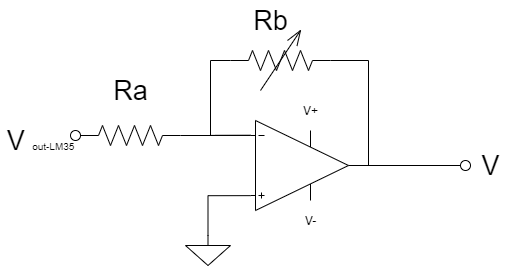
\includegraphics[scale=0.5]{../Ejercicio4-CircuitodeAplicacion/CircInversor.png}
    \caption{Circuito Inversor}
\end{figure}

Por lo tanto el circuito de aplicación será el siguiente:

\begin{figure}[H]
    \centering
    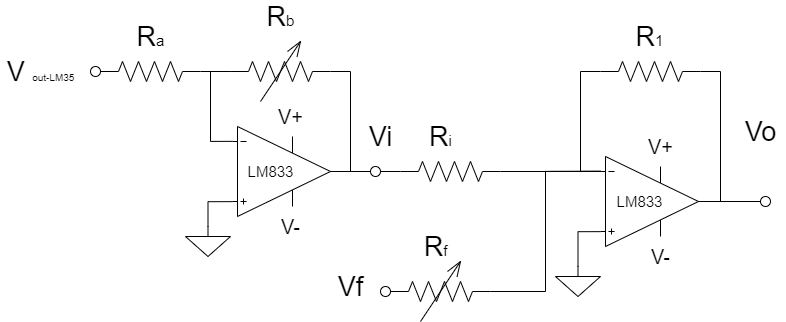
\includegraphics[scale=0.5]{../Ejercicio4-CircuitodeAplicacion/CircAplicacion.png}
    \caption{Esquema del Circuito propuesto}
\end{figure}


\subsection{Limitación de tensión en la salida}

Se nos pide implementar un circuito de protección para que la salida se mantenga en un rango $-1V < V_o < 6V$, para asegurar este rango se implemento un diodo a la salida a modo de regulador de tensión. En particular se eligió un diodo Zener 1N750 el cual limita la tensión positiva con una tensión de ruptura cerca de $5,6V$ mientras que en las tensiones negativas tiene una tensión de directa de $-0,7V$. Con esta protección se cumplen los requisitos impuestos. El circuito final será:

\begin{figure}[H]
    \centering
    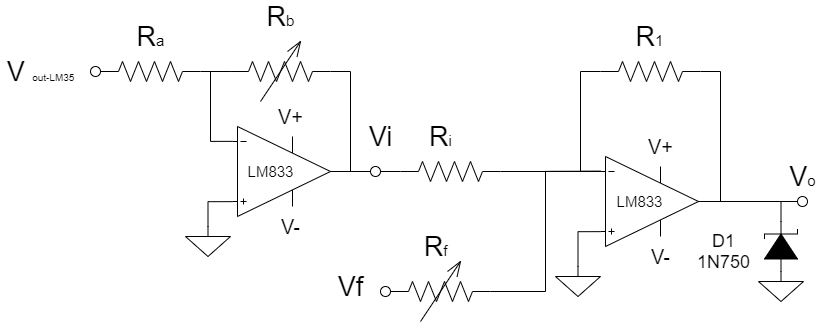
\includegraphics[scale=0.5]{../Ejercicio4-CircuitodeAplicacion/CircProteccion.png}
    \caption{Circuito con protección}
\end{figure}


\subsection{Hoja de datos relevantes}





\end{document}